% Scoping Review Outline — Gut Microbiome and Time-to-GVHD in Adult Allo-SCT
% This is a working outline with figure placeholders and bullet-point content guides.
% Compile with: pdflatex -> biber -> pdflatex -> pdflatex
%%%%%%%%%%%%%%%%%%%%%%%%%%%%%%%%%%%%%%%%%%%%%%%%%%%%%%%%%%%%%%%%%%%

\documentclass[11pt,a4paper]{article}
\usepackage[margin=2.5cm]{geometry}
\usepackage[onehalfspacing]{setspace}
\usepackage{graphicx}
\usepackage[breaklinks=true,colorlinks=true,linkcolor=blue,urlcolor=blue,citecolor=blue]{hyperref}
\usepackage{amsmath,amssymb}
\usepackage[T1]{fontenc}
\usepackage{booktabs}
\usepackage{longtable}
\usepackage{array}
\usepackage{xcolor}
\usepackage{tikz}
\usetikzlibrary{shapes.geometric, arrows.meta, positioning, calc, fit, backgrounds}
\usepackage{tabularray}
\usepackage{enumitem}

% Bibliography
\usepackage[backend=biber, style=numeric, sorting=none, autocite=superscript, maxnames=10]{biblatex}
\addbibresource{references.bib}

% Custom commands for outline mode
\newcommand{\todoitem}[1]{\textcolor{blue!70!black}{\textbullet~#1}}
\newcommand{\writingnote}[1]{\par\noindent\colorbox{yellow!30}{\parbox{\dimexpr\linewidth-2\fboxsep}{%
  \small\textbf{Writing note:} #1}}\par\medskip}
\newcommand{\placeholder}[1]{\par\noindent\colorbox{gray!15}{\parbox{\dimexpr\linewidth-2\fboxsep}{%
  \small\textit{#1}}}\par\medskip}

\graphicspath{{Bilder/}{images/}{../AnalyticCohort/images/}{../AnalyticCohort/}{../AnalyticCohort/Uncorrected/}{../AnalyticCohort/CombatSeq/}}


%%%%%%%%%%%%%%%%%%%%%%%%%%%%%%%%%%%%%%%%%%%%%%%%%%%%%%%%%%%%%%%%%%%
\begin{document}

\title{Gut Microbiome and Time-to-GVHD in Adult Allogeneic\\
Stem Cell Transplant Recipients:\\
A Scoping Review and Description of an Analytic Cohort}
\author{Sophie Huebler\thanks{\href{mailto:sophie.huebler@utah.edu}{sophie.huebler@utah.edu}}}
\date{\today~--- \textcolor{red}{WORKING OUTLINE}}
\maketitle

\renewcommand\abstractname{Abstract}
\begin{abstract}
\noindent\textbf{Background:}
\todoitem{Targeted microbiome therapies (designer microbiomes, phage-derived enzymes) now exist, making identification of specific microbial targets clinically actionable.}
\todoitem{Many narrative reviews exist but evidence base has not been quantitatively mapped.}

\noindent\textbf{Objectives:}
\todoitem{(1) Conduct a scoping review of gut microbiome studies in adult allo-SCT cohorts with GVHD outcomes.}
\todoitem{(2) Build a citation network to quantify independent replication of key claims.}
\todoitem{(3) Describe an analytic sub-cohort of studies with time-to-GVHD data and publicly available 16S sequencing.}

\noindent\textbf{Eligibility Criteria:}
\todoitem{Adult ($\geq$18) allo-HSCT, gut microbiome (16S or shotgun), GVHD outcome, original research.}

\noindent\textbf{Sources and Methods:}
\todoitem{PRISMA-ScR framework. PubMed, Embase, Web of Science. Citation network analysis of review papers.}

\noindent\textbf{Results:}
\todoitem{[N] studies included. Citation network reveals [key finding about replication]. Analytic sub-cohort: [N] studies, [N] patients.}

\noindent\textbf{Conclusions:}
\todoitem{Evidence thinner than citation frequency suggests. Time-to-GVHD understudied. Analytic cohort provides resource for further statistical investigation.}
\end{abstract}

\tableofcontents
\newpage


%===================================================================
\section{Introduction}
\label{sec:introduction}
%===================================================================

\writingnote{Structure: therapeutic motivation $\to$ gap identification $\to$ objectives. Aim for 4--5 paragraphs.}

\subsection*{Paragraph 1: The therapeutic pipeline}
\todoitem{Open with the clinical stakes: GVHD is a leading cause of morbidity/mortality after allo-HSCT.}
\todoitem{Introduce targeted microbiome therapies as a motivating frame: designer microbiomes, FMT, phage-derived enzymes.}
\todoitem{Cite Fujimoto2024 as a concrete example --- anti-\textit{E.~faecalis} enzyme developed to target a specific GVHD-associated pathogen.}
\todoitem{Key message: once a microbial target is identified, intervention is increasingly feasible.}

\subsection*{Paragraph 2: What is currently known}
\todoitem{Reduced alpha diversity broadly associated with worse GVHD outcomes.}
\todoitem{Specific taxa repeatedly mentioned: \textit{Blautia}, \textit{Enterococcus}, \textit{Lachnospiraceae}, \textit{Ruminococcaceae}.}
\todoitem{Metabolite pathways: SCFAs (butyrate), bile acids.}
\todoitem{These findings cited across many reviews --- but how independently replicated are they?}

\subsection*{Paragraph 3: The citation amplification problem}
\todoitem{20+ narrative/clinical reviews exist on gut microbiome and GVHD (cite representative set from Table~\ref{tab:tier4}).}
\todoitem{A single influential study may be cited by many reviews, which then cite each other.}
\todoitem{This creates an appearance of broad consensus that may rest on very few independent cohorts.}
\todoitem{No prior work has quantitatively mapped the evidence base to distinguish genuine replication from citation echo.}

\subsection*{Paragraph 4: Time-to-GVHD as an understudied outcome}
\todoitem{Most studies report GVHD occurrence (yes/no); fewer model time-to-event.}
\todoitem{Time-to-GVHD is more clinically informative and enables competing risks analysis (death, relapse).}
\todoitem{Publicly available datasets with both time-to-GVHD and microbiome data are scarce.}

\subsection*{Paragraph 5: Objectives}
\todoitem{State the three objectives formally:}
\begin{enumerate}[label=(\arabic*)]
    \item Conduct a scoping review following PRISMA-ScR guidelines to map the evidence landscape.
    \item Build a citation network to quantify independent replication of commonly-cited claims.
    \item Describe an analytic sub-cohort of adult allo-SCT studies with time-to-GVHD outcomes and publicly available 16S data, harmonized via a standardized QIIME2 pipeline.
\end{enumerate}


%===================================================================
\section{Methods}
\label{sec:methods}
%===================================================================

%-------------------------------------------------------------------
\subsection{Protocol and Registration}
\label{sec:protocol}
%-------------------------------------------------------------------
\todoitem{This scoping review was conducted in accordance with the PRISMA-ScR (Preferred Reporting Items for Systematic Reviews and Meta-Analyses extension for Scoping Reviews) guidelines.}
\todoitem{AI tool use is reported following the \textbf{PRISMA-trAIce} checklist \cite{PRISMAtrAIce2025} --- the extension to PRISMA 2020 for transparent reporting of AI as a \emph{methodological tool} in evidence synthesis. This is distinct from PRISMA-AI \cite{PRISMAAI2023}, which covers systematic reviews \emph{of} AI interventions.}
\todoitem{The protocol was not pre-registered. Rationale: scoping review, not systematic review; no meta-analytic synthesis.}

%-------------------------------------------------------------------
\subsection{Eligibility Criteria}
\label{sec:eligibility}
%-------------------------------------------------------------------

\writingnote{Use PCC framework (Population, Concept, Context) standard for scoping reviews.}

\todoitem{\textbf{Population:} Adult ($\geq$18 years) recipients of allogeneic hematopoietic stem cell transplantation. Pediatric cohorts included in the scoping review (flagged) but excluded from the analytic sub-cohort.}

\todoitem{\textbf{Concept:} Gut microbiome composition assessed by 16S rRNA gene sequencing or shotgun metagenomics.}

\todoitem{\textbf{Context:} GVHD reported as an outcome (acute or chronic; occurrence, timing, and/or severity).}

\todoitem{\textbf{Study types included:} Original observational studies, clinical trials, cohort studies.}

\todoitem{\textbf{Excluded:} Narrative reviews, editorials, conference abstracts, case reports ($n<5$), animal-only studies, studies with no GVHD outcome.}

%-------------------------------------------------------------------
\subsection{Information Sources and Search Strategy}
\label{sec:search}
%-------------------------------------------------------------------
\todoitem{Databases: PubMed, Embase, Web of Science.}
\todoitem{Date range: inception through [search date, 2026].}
\todoitem{Search string: [document the full Boolean query].}
\todoitem{Supplementary: hand-searching reference lists of all included reviews.}

\placeholder{Full search strategy to be included as Supplementary Table S1.}

%-------------------------------------------------------------------
\subsection{Use of Artificial Intelligence}
\label{sec:ai_use}
%-------------------------------------------------------------------

\writingnote{Required by PRISMA-trAIce. Report tool name, version, prompts, human--AI interaction model, and performance metrics for each stage. All records logged in \texttt{AI\_assisted\_litreview/}.}

\todoitem{\textbf{AI tool:} Claude [version] (Anthropic). All sessions logged with date, prompts, and outputs in \texttt{AI\_assisted\_litreview/logs/}.}

\todoitem{\textbf{Title/abstract screening:} AI performed initial pass against documented eligibility criteria using the prompt provided in Supplementary Table S3. Human reviewer independently screened a random [10\%] validation subsample; sensitivity and specificity of AI screening reported in Table~\ref{tab:ai_performance}. All AI ``include'' and ``uncertain'' decisions were reviewed by a human reviewer. Disagreements resolved by [method].}

\todoitem{\textbf{Full-text screening:} Human reviewer made all final include/exclude decisions. AI was used to flag potential exclusion reasons for human confirmation. All AI-generated flags were verified by the human reviewer.}

\todoitem{\textbf{Data extraction:} AI generated a structured first-pass draft of the data extraction table from full-text PDFs. Human reviewer verified every field against the source document. Discrepancies and corrections are logged in \texttt{AI\_assisted\_litreview/logs/}.}

\todoitem{\textbf{Citation network construction:} Automated via R/Python scripts (see \texttt{AI\_assisted\_litreview/prompts/citation\_network.md}). Reference lists were parsed programmatically; the citation network was constructed computationally (igraph/networkx), not by LLM inference. Human review of network outputs performed before finalization.}

\todoitem{\textbf{AI performance (title/abstract screening):}}

\begin{table}[htbp]
\centering
\caption{\textbf{AI screening performance on validation sample.} \textcolor{red}{To be filled after screening is complete.}}
\label{tab:ai_performance}
\small
\begin{tabular}{@{}lcc@{}}
\toprule
Metric & Value & 95\% CI \\
\midrule
Validation sample size & \textcolor{red}{??} & --- \\
Sensitivity (recall) & \textcolor{red}{??} & \textcolor{red}{??} \\
Specificity & \textcolor{red}{??} & \textcolor{red}{??} \\
Cohen's $\kappa$ (AI vs.\ human) & \textcolor{red}{??} & \textcolor{red}{??} \\
AI workload reduction & \textcolor{red}{??}\% & --- \\
\bottomrule
\end{tabular}
\end{table}

%-------------------------------------------------------------------
\subsection{Study Selection and Data Extraction}
\label{sec:extraction}
%-------------------------------------------------------------------
\todoitem{Two-stage screening: title/abstract, then full-text review.}
\todoitem{Structured data extraction form capturing:}
\begin{itemize}[nosep]
    \item Study design, sample size, geographic region, year
    \item Microbiome platform (16S variable region, sequencing technology, bioinformatic pipeline)
    \item Sample timing / baseline definition
    \item GVHD outcome type (acute/chronic, occurrence/timing/severity)
    \item Key findings (taxa, diversity metrics, metabolite pathways)
    \item Data availability (public repository, accession number)
\end{itemize}

\todoitem{Studies categorized into four tiers:}
\begin{itemize}[nosep]
    \item Tier 1: Reanalysis-ready (raw reads + complete clinical metadata with GVHD outcomes)
    \item Tier 2: Salvageable (raw reads exist but metadata incomplete)
    \item Tier 3: Summary-only (no raw reads, but usable summary statistics)
    \item Tier 4: Narrative/review (relevant conceptually, no extractable quantitative data)
\end{itemize}

%-------------------------------------------------------------------
\subsection{Citation Network Analysis}
\label{sec:citation_network}
%-------------------------------------------------------------------

\writingnote{This is the novel methodological contribution. Describe clearly enough that it is reproducible.}

\todoitem{Compile complete reference lists from all included Tier 4 narrative/clinical reviews.}
\todoitem{For each commonly-cited empirical claim (e.g., ``\textit{Blautia} associated with reduced GVHD''), trace the citation chain from reviews back to the original empirical study(ies).}
\todoitem{Construct a bipartite network: review papers $\to$ primary empirical studies they cite.}
\todoitem{Compute:}
\begin{itemize}[nosep]
    \item Review citation frequency for each primary study (how many reviews cite it)
    \item Independent replication count for each claim (how many distinct cohorts support it)
    \item Citation amplification ratio = (number of reviews citing a claim) / (number of independent cohorts supporting it)
\end{itemize}
\todoitem{Network visualization generated using [R/igraph or Python/networkx].}

%-------------------------------------------------------------------
\subsection{Analytic Sub-Cohort Selection and Harmonization}
\label{sec:subcohort_methods}
%-------------------------------------------------------------------
\todoitem{Additional inclusion criteria beyond the scoping review:}
\begin{itemize}[nosep]
    \item Time-to-GVHD outcome available (not just occurrence)
    \item Publicly available 16S rRNA sequencing data with accession number
    \item Individual-level clinical metadata accessible
\end{itemize}

\todoitem{Baseline definition: closest available stool sample to day 0 of transplant. Document deviations by study (e.g., pre-conditioning samples in Allozithro).}

\todoitem{Harmonization pipeline: all raw reads reprocessed through a standardized QIIME2 pipeline (DADA2 denoising, SILVA classifier, phylogenetic tree construction). Batch correction assessed using ComBat-seq.}


%===================================================================
\section{Results}
\label{sec:results}
%===================================================================

%-------------------------------------------------------------------
\subsection{Search Results and Study Selection}
\label{sec:prisma}
%-------------------------------------------------------------------

%%% FIGURE 1: PRISMA-trAIce MODIFIED FLOW DIAGRAM %%%
% Modified per PRISMA-trAIce (2025): AI exclusions and human exclusions tracked separately.
% AI steps shown in purple/violet; human steps in standard blue/green.
\begin{figure}[htbp]
\centering
\resizebox{\textwidth}{!}{%
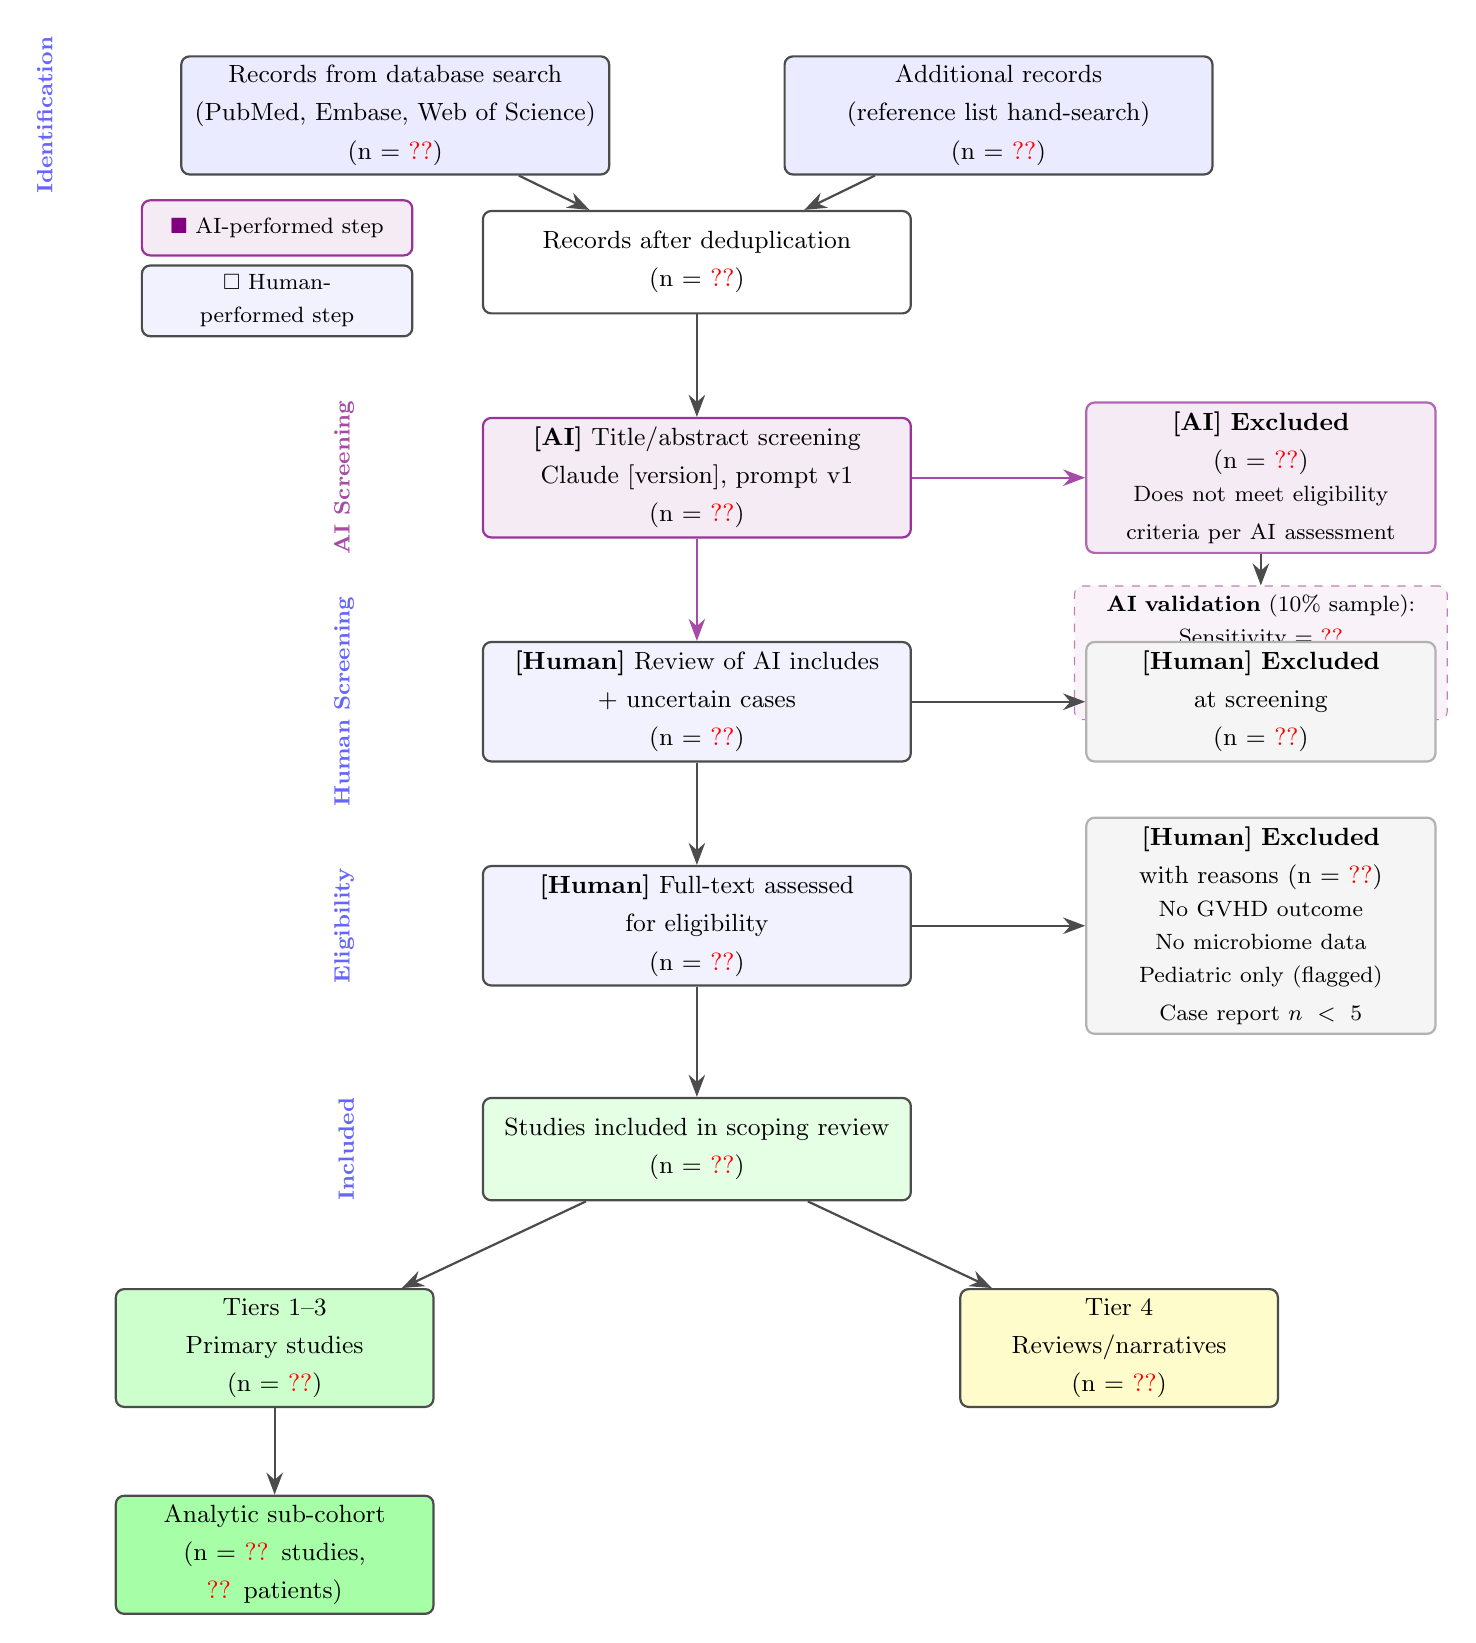
\begin{tikzpicture}[
    % Standard PRISMA boxes (human decisions)
    box/.style={rectangle, draw=black!70, thick, rounded corners=3pt,
                text width=5.2cm, minimum height=1.3cm, align=center, font=\small},
    % AI-step boxes (violet border, light fill)
    aibox/.style={rectangle, draw=violet!80, thick, rounded corners=3pt,
                  text width=5.2cm, minimum height=1.3cm, align=center,
                  font=\small, fill=violet!8},
    % Exclusion side-boxes
    excbox/.style={rectangle, draw=gray!60, thick, rounded corners=3pt,
                   text width=4.2cm, minimum height=1.1cm, align=center,
                   font=\small, fill=gray!8},
    % AI exclusion side-boxes (violet)
    aiexcbox/.style={rectangle, draw=violet!60, thick, rounded corners=3pt,
                     text width=4.2cm, minimum height=1.1cm, align=center,
                     font=\small, fill=violet!8},
    % Performance note box
    notebox/.style={rectangle, draw=violet!50, dashed, rounded corners=3pt,
                    text width=4.5cm, align=center, font=\footnotesize,
                    fill=violet!5},
    arrow/.style={-{Stealth[length=2.8mm]}, thick, black!70},
    aiarrow/.style={-{Stealth[length=2.8mm]}, thick, violet!70},
    node distance=1.3cm
]

%-------- IDENTIFICATION --------
\node[box, fill=blue!8] (id) {Records from database search\\(PubMed, Embase, Web of Science)\\(n~=~\textcolor{red}{??})};
\node[box, fill=blue!8, right=2.2cm of id] (other) {Additional records\\(reference list hand-search)\\(n~=~\textcolor{red}{??})};
\node[box, below=1.2cm of $(id)!0.5!(other)$] (dedup) {Records after deduplication\\(n~=~\textcolor{red}{??})};

%-------- SCREENING: AI STAGE --------
\node[aibox, below=of dedup] (aiscreen)
    {\textbf{[AI]} Title/abstract screening\\
     Claude [version], prompt v1\\
     (n~=~\textcolor{red}{??})};
\node[aiexcbox, right=2.2cm of aiscreen] (aiexcl)
    {\textbf{[AI] Excluded}\\
     (n~=~\textcolor{red}{??})\\
     {\footnotesize Does not meet eligibility\\criteria per AI assessment}};
\node[notebox, below=0.4cm of aiexcl] (aiperf)
    {\textbf{AI validation} (10\% sample):\\
     Sensitivity~=~\textcolor{red}{??}\\
     Specificity~=~\textcolor{red}{??}\\
     $\kappa$~=~\textcolor{red}{??}};

%-------- SCREENING: HUMAN VERIFICATION --------
\node[box, fill=blue!5, below=of aiscreen] (humanscreen)
    {\textbf{[Human]} Review of AI includes\\
     + uncertain cases\\
     (n~=~\textcolor{red}{??})};
\node[excbox, right=2.2cm of humanscreen] (humanexcl)
    {\textbf{[Human] Excluded}\\
     at screening\\
     (n~=~\textcolor{red}{??})};

%-------- ELIGIBILITY: FULL-TEXT --------
\node[box, fill=blue!5, below=of humanscreen] (elig)
    {\textbf{[Human]} Full-text assessed\\
     for eligibility\\
     (n~=~\textcolor{red}{??})};
\node[excbox, right=2.2cm of elig] (excl2)
    {\textbf{[Human] Excluded}\\
     with reasons (n~=~\textcolor{red}{??})\\
     {\footnotesize No GVHD outcome\\
     No microbiome data\\
     Pediatric only (flagged)\\
     Case report $n<5$}};

%-------- INCLUDED --------
\node[box, fill=green!10, below=1.4cm of elig] (incl)
    {Studies included in scoping review\\(n~=~\textcolor{red}{??})};

%-------- TIERS --------
\node[box, fill=green!20, below left=1.1cm and 0.6cm of incl, text width=3.8cm]
    (t13) {Tiers 1--3\\Primary studies\\(n~=~\textcolor{red}{??})};
\node[box, fill=yellow!20, below right=1.1cm and 0.6cm of incl, text width=3.8cm]
    (t4)  {Tier 4\\Reviews/narratives\\(n~=~\textcolor{red}{??})};

%-------- ANALYTIC SUB-COHORT --------
\node[box, fill=green!35, below=1.1cm of t13, text width=3.8cm]
    (sub) {Analytic sub-cohort\\(n~=~\textcolor{red}{??} studies,\\\textcolor{red}{??} patients)};

%-------- ARROWS: main flow --------
\draw[arrow] (id)          -- (dedup);
\draw[arrow] (other)       -- (dedup);
\draw[arrow] (dedup)       -- (aiscreen);
\draw[aiarrow] (aiscreen)  -- (humanscreen);
\draw[arrow]  (humanscreen)-- (elig);
\draw[arrow]  (elig)       -- (incl);
\draw[arrow]  (incl)       -- (t13);
\draw[arrow]  (incl)       -- (t4);
\draw[arrow]  (t13)        -- (sub);

%-------- ARROWS: exclusions --------
\draw[aiarrow] (aiscreen)    -- (aiexcl);
\draw[arrow]   (aiexcl)      -- (aiperf);
\draw[arrow]   (humanscreen) -- (humanexcl);
\draw[arrow]   (elig)        -- (excl2);

%-------- PHASE LABELS --------
\node[rotate=90, anchor=south, font=\footnotesize\bfseries, text=blue!60]
    at ($(id.west)+(-1.5,0)$)          {Identification};
\node[rotate=90, anchor=south, font=\footnotesize\bfseries, text=violet!70]
    at ($(aiscreen.west)+(-1.5,0)$)    {AI Screening};
\node[rotate=90, anchor=south, font=\footnotesize\bfseries, text=blue!60]
    at ($(humanscreen.west)+(-1.5,0)$) {Human Screening};
\node[rotate=90, anchor=south, font=\footnotesize\bfseries, text=blue!60]
    at ($(elig.west)+(-1.5,0)$)        {Eligibility};
\node[rotate=90, anchor=south, font=\footnotesize\bfseries, text=blue!60]
    at ($(incl.west)+(-1.5,0)$)        {Included};

%-------- LEGEND --------
\node[box, fill=violet!8, draw=violet!80, text width=3.2cm, minimum height=0.7cm,
      font=\footnotesize, anchor=north west]
    at ($(id.south west)+(-0.5,-0.3)$) (leg_ai)
    {\textcolor{violet}{$\blacksquare$} AI-performed step};
\node[box, fill=blue!5, draw=black!70, text width=3.2cm, minimum height=0.7cm,
      font=\footnotesize, anchor=north west]
    at ($(leg_ai.south west)+(0,-0.1)$)
    {$\square$ Human-performed step};

\end{tikzpicture}
}% end resizebox
\caption{\textbf{PRISMA-trAIce modified flow diagram.}
Study identification, screening, and inclusion process following PRISMA-ScR guidelines with the PRISMA-trAIce extension for transparent AI reporting.
Violet nodes represent steps performed by AI (Claude); blue nodes represent human-performed steps.
The screening stage is split per PRISMA-trAIce requirements: AI exclusions and human exclusions are tracked separately.
The AI validation box reports screening performance on a random 10\% human gold-standard subsample.
Numbers to be filled after search and screening are complete.
Studies are categorized into Tiers 1--4; the analytic sub-cohort additionally requires time-to-GVHD outcomes and publicly available 16S data.}
\label{fig:prisma}
\end{figure}


\todoitem{Report total records identified, deduplicated, screened, included.}
\todoitem{Breakdown by tier.}
\todoitem{Common exclusion reasons.}


%-------------------------------------------------------------------
\subsection{Characteristics of Included Studies}
\label{sec:characteristics}
%-------------------------------------------------------------------

%%% TABLE 1: STUDY CHARACTERISTICS %%%
\begin{table}[htbp]
\centering
\caption{\textbf{Characteristics of included primary studies.} \textcolor{red}{Placeholder --- to be populated after search/extraction.}}
\label{tab:characteristics}
\small
\begin{tabular}{@{}lccccccl@{}}
\toprule
Study & Year & $N$ & Design & 16S Region & Baseline & GVHD Outcome & Accession \\
\midrule
\textcolor{gray}{Bergeron (Allozithro)} & \textcolor{gray}{2017} & \textcolor{gray}{50} & \textcolor{gray}{RCT} & \textcolor{gray}{V3--V4} & \textcolor{gray}{Day 0} & \textcolor{gray}{a/c, time} & \textcolor{gray}{PRJNA902819} \\
\textcolor{gray}{Liu} & \textcolor{gray}{2017} & \textcolor{gray}{57} & \textcolor{gray}{Prospective} & \textcolor{gray}{V3--V4} & \textcolor{gray}{Day 0} & \textcolor{gray}{a/c, time} & \textcolor{gray}{PRJEB16057} \\
\textcolor{gray}{Fujimoto} & \textcolor{gray}{2024} & \textcolor{gray}{46?} & \textcolor{gray}{Retrospective} & \textcolor{gray}{V3--V4?} & \textcolor{gray}{Pre-cond.} & \textcolor{gray}{a, occurrence} & \textcolor{gray}{PRJNA1109929} \\
\textcolor{red}{[additional studies]} & & & & & & & \\
\textcolor{red}{$\vdots$} & & & & & & & \\
\bottomrule
\end{tabular}
\end{table}

\todoitem{Summary paragraph: geographic distribution, year range, sample size range, most common sequencing platforms.}
\todoitem{Describe heterogeneity in baseline definitions across studies --- this is a key finding.}


%-------------------------------------------------------------------
\subsection{Citation Network and Evidence Mapping}
\label{sec:citation_results}
%-------------------------------------------------------------------

\writingnote{This section presents the paper's most novel contribution. Two outputs: the citation network figure and the evidence table.}

%%% FIGURE 2: CITATION NETWORK %%%
\begin{figure}[htbp]
\centering
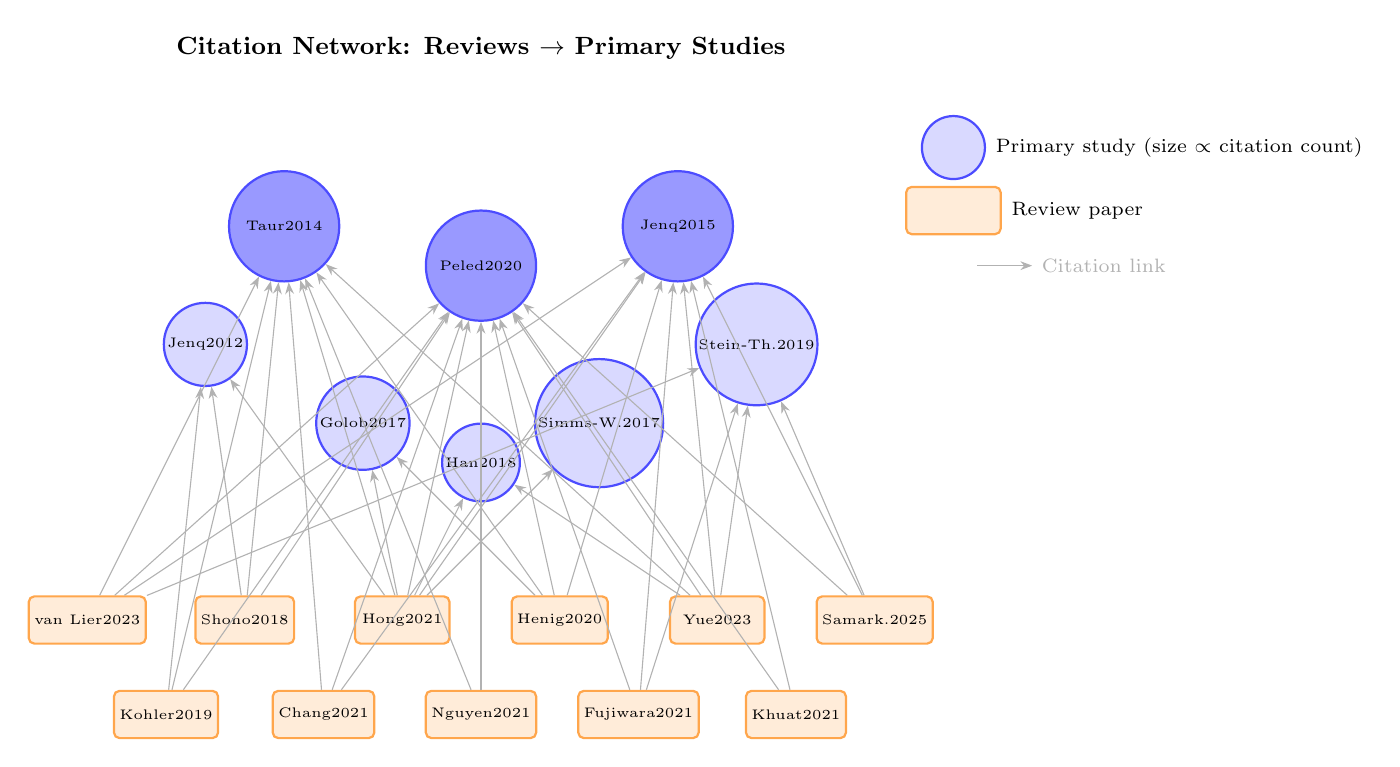
\begin{tikzpicture}[
    primary/.style={circle, draw=blue!70, thick, fill=blue!15,
                    minimum size=8mm, font=\tiny, inner sep=1pt},
    primarybig/.style={circle, draw=blue!70, thick, fill=blue!40,
                       minimum size=14mm, font=\tiny, inner sep=1pt},
    review/.style={rectangle, draw=orange!70, thick, fill=orange!15,
                   rounded corners=2pt, minimum width=12mm, minimum height=6mm,
                   font=\tiny, inner sep=2pt},
    cite/.style={-{Stealth[length=1.5mm]}, gray!60, thin},
]

% Title
\node[font=\small\bfseries, anchor=south] at (0,5) {Citation Network: Reviews $\to$ Primary Studies};

% Primary studies (circles, sized by citation count)
\node[primarybig] (peled) at (0,2.5) {Peled\\2020};
\node[primarybig] (taur) at (-2.5,3) {Taur\\2014};
\node[primarybig] (jenq15) at (2.5,3) {Jenq\\2015};
\node[primary] (jenq12) at (-3.5,1.5) {Jenq\\2012};
\node[primary] (stein) at (3.5,1.5) {Stein-Th.\\2019};
\node[primary] (golob) at (-1.5,0.5) {Golob\\2017};
\node[primary] (simms) at (1.5,0.5) {Simms-W.\\2017};
\node[primary] (han18) at (0,0) {Han\\2018};

% Review papers (rectangles, bottom)
\node[review] at (-5,-2) (r1) {van Lier\\2023};
\node[review] at (-3,-2) (r2) {Shono\\2018};
\node[review] at (-1,-2) (r3) {Hong\\2021};
\node[review] at (1,-2) (r4) {Henig\\2020};
\node[review] at (3,-2) (r5) {Yue\\2023};
\node[review] at (5,-2) (r6) {Samark.\\2025};
\node[review] at (-4,-3.2) (r7) {Kohler\\2019};
\node[review] at (-2,-3.2) (r8) {Chang\\2021};
\node[review] at (0,-3.2) (r9) {Nguyen\\2021};
\node[review] at (2,-3.2) (r10) {Fujiwara\\2021};
\node[review] at (4,-3.2) (r11) {Khuat\\2021};

% Citation edges (reviews -> primary)
% Peled (cited by many)
\foreach \r in {r1,r2,r3,r4,r5,r6,r7,r8,r9,r10,r11} {
    \draw[cite] (\r) -- (peled);
}
% Taur (cited by many)
\foreach \r in {r1,r2,r3,r4,r5,r7,r8,r9} {
    \draw[cite] (\r) -- (taur);
}
% Jenq2015 (cited by many)
\foreach \r in {r1,r3,r4,r5,r6,r8,r10,r11} {
    \draw[cite] (\r) -- (jenq15);
}
% Jenq2012 (fewer)
\foreach \r in {r2,r3,r7} {
    \draw[cite] (\r) -- (jenq12);
}
% Stein-Thoeringer
\foreach \r in {r1,r5,r6,r10} {
    \draw[cite] (\r) -- (stein);
}
% Golob
\foreach \r in {r3,r4} {
    \draw[cite] (\r) -- (golob);
}
% Simms-Waldrip
\foreach \r in {r3} {
    \draw[cite] (\r) -- (simms);
}
% Han
\foreach \r in {r3,r5} {
    \draw[cite] (\r) -- (han18);
}

% Legend
\node[primary, label=right:{\scriptsize Primary study (size $\propto$ citation count)}] at (6,4) {};
\node[review, label=right:{\scriptsize Review paper}] at (6,3.2) {};
\draw[cite] (6.3,2.5) -- (7,2.5) node[right, font=\scriptsize] {Citation link};

\end{tikzpicture}
\caption{\textbf{Citation network} showing the relationship between narrative/clinical review papers (orange rectangles) and the primary empirical studies they cite (blue circles). Node size for primary studies is proportional to the number of reviews citing that study. \textcolor{red}{Placeholder layout --- node positions, sizes, and edges will be computed from actual reference data. Illustrative only.}}
\label{fig:citation_network}
\end{figure}


%%% TABLE 2: EVIDENCE MAP %%%
\begin{table}[htbp]
\centering
\caption{\textbf{Evidence map: commonly-cited claims traced to independent empirical sources.} The citation amplification ratio quantifies how much review citation frequency exceeds independent replication. \textcolor{red}{Placeholder values --- to be populated from citation network analysis.}}
\label{tab:evidence_map}
\small
\renewcommand{\arraystretch}{1.3}
\begin{tabular}{@{}p{4cm}p{3.5cm}cp{2.8cm}@{}}
\toprule
Claim & Independent cohorts & \# Reviews & Amplification \\
 & (primary sources) & citing & ratio \\
\midrule
Reduced $\alpha$-diversity $\to$ aGVHD risk & \textcolor{red}{Taur 2014, Jenq 2015, Peled 2020, [?]} & \textcolor{red}{15/20} & \textcolor{red}{$\sim$5:1} \\
\addlinespace
\textit{Blautia} $\to$ reduced GVHD mortality & \textcolor{red}{Jenq 2015, [?]} & \textcolor{red}{12/20} & \textcolor{red}{$\sim$6--12:1} \\
\addlinespace
\textit{Enterococcus} domination $\to$ aGVHD & \textcolor{red}{Stein-Th. 2019, [?]} & \textcolor{red}{10/20} & \textcolor{red}{$\sim$5--10:1} \\
\addlinespace
\textit{Lachnospiraceae} depletion $\to$ worse outcomes & \textcolor{red}{[?]} & \textcolor{red}{?/20} & \textcolor{red}{?} \\
\addlinespace
Butyrate/SCFA pathways $\to$ GVHD protection & \textcolor{red}{[?]} & \textcolor{red}{?/20} & \textcolor{red}{?} \\
\addlinespace
Antibiotic-driven dysbiosis $\to$ GVHD & \textcolor{red}{Simms-Waldrip 2017, [?]} & \textcolor{red}{?/20} & \textcolor{red}{?} \\
\bottomrule
\end{tabular}
\end{table}

\todoitem{Narrative paragraph interpreting the citation network: which claims are robustly supported vs. resting on 1--2 cohorts.}
\todoitem{Highlight the most striking amplification ratios.}
\todoitem{Note which primary studies are ``load-bearing'' across the review literature (e.g., Peled 2020 cited by nearly all reviews).}


%-------------------------------------------------------------------
\subsection{Synthesis of Findings by Theme}
\label{sec:synthesis}
%-------------------------------------------------------------------

\writingnote{Organize by claim/theme, not by study. Reference the evidence table (Table~\ref{tab:evidence_map}) throughout. For each theme, report what the independent evidence actually shows, stripped of citation amplification.}

\subsubsection{Alpha Diversity and GVHD Risk}
\todoitem{Summarize the independent evidence for the diversity--GVHD association.}
\todoitem{Note the diversity metrics used (Shannon, inverse Simpson, observed ASVs) and whether they converge.}
\todoitem{Distinguish diversity at different timepoints (pre-transplant vs.\ engraftment vs.\ post-transplant).}

\subsubsection{Specific Taxa Associated with GVHD Outcomes}
\todoitem{\textit{Blautia}: trace to original finding (Jenq 2015). How many independent cohorts have replicated?}
\todoitem{\textit{Enterococcus}: Stein-Thoeringer 2019 (lactose-driven expansion). Replicated in which cohorts?}
\todoitem{\textit{Lachnospiraceae} and \textit{Ruminococcaceae}: trace evidence.}
\todoitem{Other taxa reported in $\geq$2 independent cohorts.}

\subsubsection{Metabolite Pathways}
\todoitem{SCFAs/butyrate: mechanistic evidence vs.\ observational replication.}
\todoitem{Bile acids: emerging evidence.}
\todoitem{Distinguish animal-model findings from human cohort evidence.}

\subsubsection{Methodological Heterogeneity}
\todoitem{Baseline/sample timing definitions across studies (this is a key finding).}
\todoitem{Sequencing platforms and 16S variable regions.}
\todoitem{Bioinformatic pipelines (OTU vs.\ ASV, reference databases).}
\todoitem{How methodological differences may explain apparent inconsistencies.}


%-------------------------------------------------------------------
\subsection{Analytic Sub-Cohort Description}
\label{sec:subcohort_results}
%-------------------------------------------------------------------

%%% TABLE 3: ANALYTIC SUB-COHORT %%%
\begin{table}[htbp]
\centering
\caption{\textbf{Studies included in the analytic sub-cohort.} All studies have publicly available 16S rRNA sequencing data and time-to-GVHD outcomes. \textcolor{red}{To be updated as additional studies are identified.}}
\label{tab:subcohort}
\small
\begin{tblr}{
  width = \linewidth,
  colspec = {Q[l,0.12] Q[c,0.05] Q[c,0.06] Q[l,0.12] Q[l,0.30] Q[c,0.10] Q[l,0.12]},
  row{1} = {font=\bfseries\small},
  hline{1,2,Z} = {0.8pt},
  cells = {font=\small},
}
Study & Year & $N$ & Design & GVHD Outcomes Available & Baseline & Accession \\
Allozithro (Bergeron) & 2017 & 50 & RCT & aGVHD (occ, sev, time), cGVHD (occ, sev, time), relapse (occ, time), death (occ, time) & Day 0 & PRJNA902819 \\
Liu & 2017 & 57 & Prospective & aGVHD (occ, sev, organ, time), cGVHD (occ, sev, time), relapse (occ, time), death (occ, time), engraftment (occ, time) & Day 0 & PRJEB16057 \\
Fujimoto & 2024 & 46? & Retrospective & aGVHD (occurrence) & Pre-cond. & PRJNA1109929 \\
\end{tblr}
\vspace{2pt}
\begin{flushleft}
\footnotesize occ = occurrence; sev = severity; time = time-to-event. $N$ = patients with 16S microbiome measurements.
\end{flushleft}
\end{table}


%%% FIGURE 3: SAMPLE INCLUSION/EXCLUSION %%%
\begin{figure}[htbp]
\centering
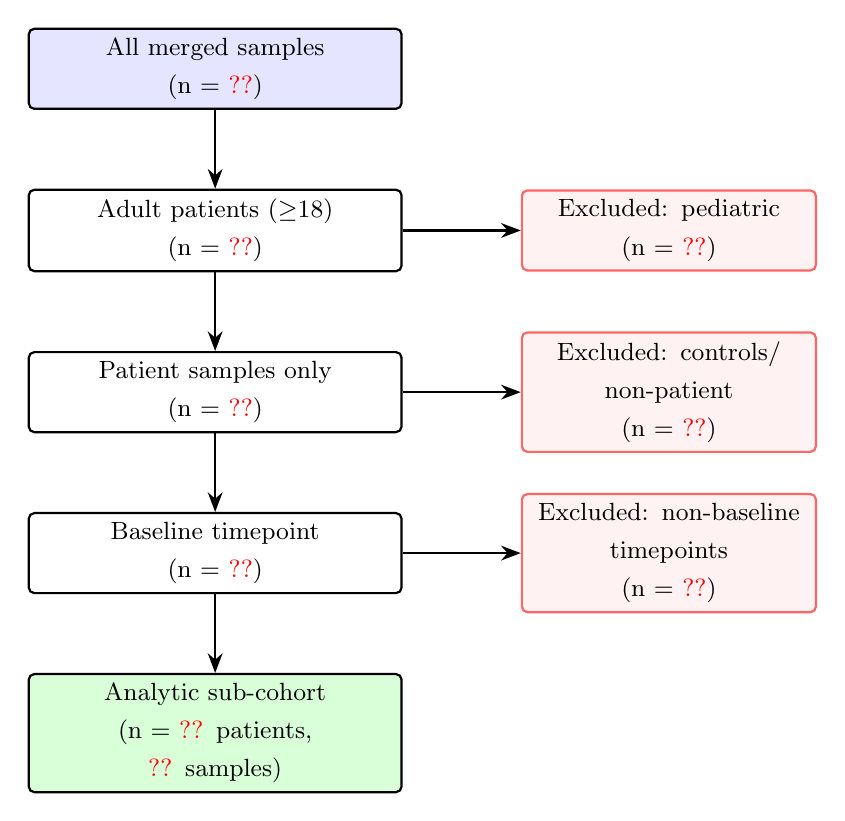
\begin{tikzpicture}[
    box/.style={rectangle, draw=black, thick, rounded corners=2pt,
                text width=4.5cm, minimum height=1cm, align=center, font=\small},
    excbox/.style={rectangle, draw=red!60, thick, rounded corners=2pt,
                   text width=3.5cm, minimum height=0.8cm, align=center,
                   font=\small, fill=red!5},
    arrow/.style={-{Stealth[length=2.5mm]}, thick},
    node distance=1cm
]

\node[box, fill=blue!10] (all) {All merged samples\\(n = \textcolor{red}{??})};
\node[box, below=of all] (adult) {Adult patients ($\geq$18)\\(n = \textcolor{red}{??})};
\node[excbox, right=1.5cm of adult] (exc1) {Excluded: pediatric\\(n = \textcolor{red}{??})};
\node[box, below=of adult] (patient) {Patient samples only\\(n = \textcolor{red}{??})};
\node[excbox, right=1.5cm of patient] (exc2) {Excluded: controls/\\non-patient\\(n = \textcolor{red}{??})};
\node[box, below=of patient] (baseline) {Baseline timepoint\\(n = \textcolor{red}{??})};
\node[excbox, right=1.5cm of baseline] (exc3) {Excluded: non-baseline\\timepoints\\(n = \textcolor{red}{??})};
\node[box, fill=green!15, below=of baseline] (final) {Analytic sub-cohort\\(n = \textcolor{red}{??} patients,\\\textcolor{red}{??} samples)};

\draw[arrow] (all) -- (adult);
\draw[arrow] (adult) -- (patient);
\draw[arrow] (patient) -- (baseline);
\draw[arrow] (baseline) -- (final);
\draw[arrow] (adult) -- (exc1);
\draw[arrow] (patient) -- (exc2);
\draw[arrow] (baseline) -- (exc3);

\end{tikzpicture}
\caption{\textbf{Sample selection for the analytic sub-cohort.} Sequential application of inclusion/exclusion criteria to the merged dataset. \textcolor{red}{Numbers to be finalized.} See also existing figure: \texttt{AnalyticCohort/images/Sample\_IncExc.png}.}
\label{fig:sample_flow}
\end{figure}


%%% FIGURE 4: COHORT COMPOSITION %%%
\begin{figure}[htbp]
\centering
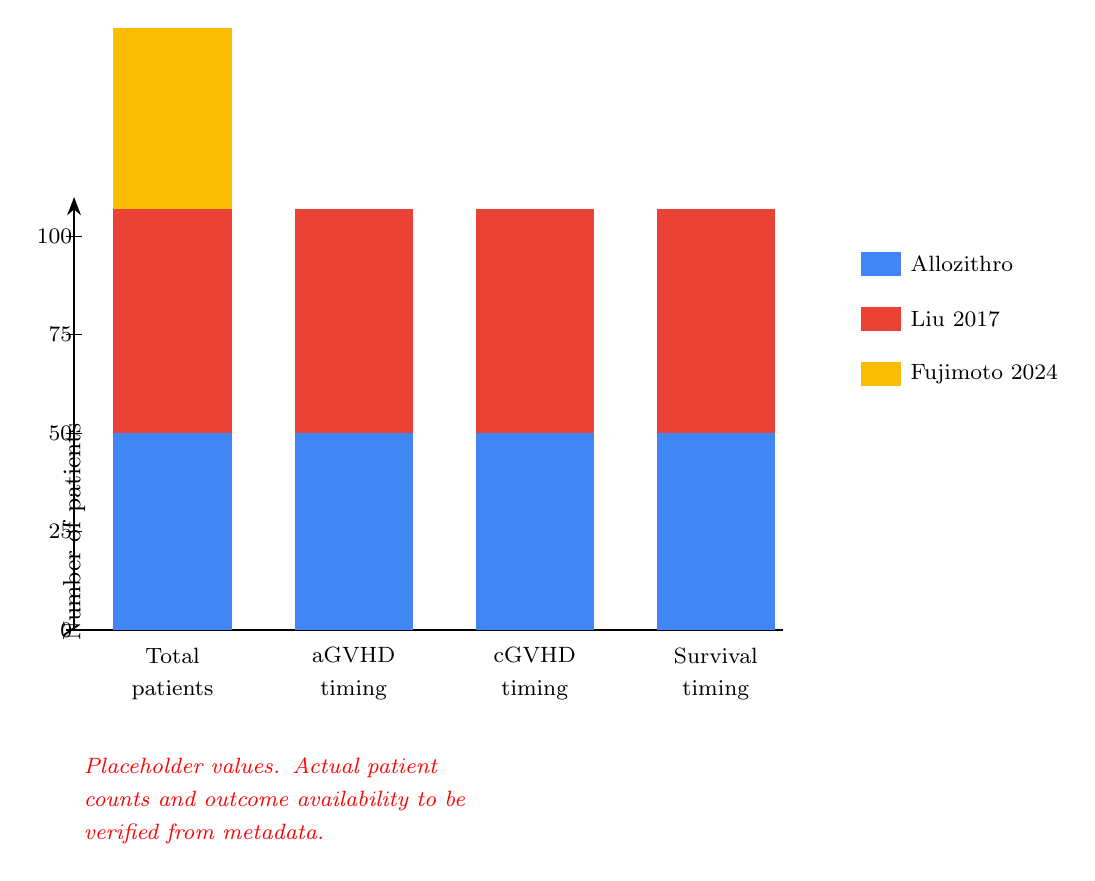
\begin{tikzpicture}
% Placeholder stacked bar chart showing study composition

\definecolor{study1}{RGB}{66,133,244}  % Blue - Allozithro
\definecolor{study2}{RGB}{234,67,53}   % Red - Liu
\definecolor{study3}{RGB}{251,188,4}   % Yellow - Fujimoto

% Axes
\draw[thick, -{Stealth}] (0,0) -- (0,5.5) node[left, rotate=90, midway, font=\small] {Number of patients};
\draw[thick] (0,0) -- (9,0);

% Bars - Study composition by outcome availability
% Bar 1: Total patients
\fill[study1] (0.5,0) rectangle (2,2.5);
\fill[study2] (0.5,2.5) rectangle (2,5.35);
\fill[study3] (0.5,5.35) rectangle (2,7.65);
\node[below, font=\footnotesize, text width=2cm, align=center] at (1.25,-0.1) {Total\\patients};

% Bar 2: With aGVHD timing
\fill[study1] (2.8,0) rectangle (4.3,2.5);
\fill[study2] (2.8,2.5) rectangle (4.3,5.35);
\node[below, font=\footnotesize, text width=2cm, align=center] at (3.55,-0.1) {aGVHD\\timing};

% Bar 3: With cGVHD timing
\fill[study1] (5.1,0) rectangle (6.6,2.5);
\fill[study2] (5.1,2.5) rectangle (6.6,5.35);
\node[below, font=\footnotesize, text width=2cm, align=center] at (5.85,-0.1) {cGVHD\\timing};

% Bar 4: With survival timing
\fill[study1] (7.4,0) rectangle (8.9,2.5);
\fill[study2] (7.4,2.5) rectangle (8.9,5.35);
\node[below, font=\footnotesize, text width=2cm, align=center] at (8.15,-0.1) {Survival\\timing};

% Y-axis ticks (approximate)
\foreach \y/\lab in {0/0, 1.25/25, 2.5/50, 3.75/75, 5/100} {
    \draw (-0.1,\y) -- (0.1,\y) node[left, font=\footnotesize] {\lab};
}

% Legend
\fill[study1] (10,4.5) rectangle (10.5,4.8);
\node[right, font=\footnotesize] at (10.5,4.65) {Allozithro};
\fill[study2] (10,3.8) rectangle (10.5,4.1);
\node[right, font=\footnotesize] at (10.5,3.95) {Liu 2017};
\fill[study3] (10,3.1) rectangle (10.5,3.4);
\node[right, font=\footnotesize] at (10.5,3.25) {Fujimoto 2024};

% Note
\node[font=\footnotesize\itshape, text width=5cm, anchor=north west] at (0,-1.5) {\textcolor{red}{Placeholder values. Actual patient counts and outcome availability to be verified from metadata.}};

\end{tikzpicture}
\caption{\textbf{Analytic sub-cohort composition} by study and outcome availability. Stacked bars show the contribution of each study to the total cohort, broken down by which time-to-event outcomes are available.}
\label{fig:cohort_composition}
\end{figure}


%%% FIGURE 5: BETA DIVERSITY %%%
\begin{figure}[htbp]
\centering
\begin{tikzpicture}

% Panel A: Uncorrected
\begin{scope}[shift={(-4.5,0)}]
    \draw[thick, -{Stealth}] (0,0) -- (0,5) node[left, rotate=90, midway, font=\small] {PC2};
    \draw[thick, -{Stealth}] (0,0) -- (6,0) node[below, midway, font=\small] {PC1};
    \node[font=\small\bfseries] at (3,5.5) {A) Uncorrected};

    % Simulated study clusters (uncorrected = separated by batch)
    \definecolor{s1}{RGB}{66,133,244}
    \definecolor{s2}{RGB}{234,67,53}
    \definecolor{s3}{RGB}{251,188,4}

    % Cluster 1 (Allozithro) - top left
    \foreach \i in {1,...,12} {
        \pgfmathsetmacro{\x}{1.2 + 0.8*rand}
        \pgfmathsetmacro{\y}{3.2 + 0.7*rand}
        \fill[s1, opacity=0.7] (\x,\y) circle (2pt);
    }
    % Cluster 2 (Liu) - bottom right
    \foreach \i in {1,...,15} {
        \pgfmathsetmacro{\x}{3.5 + 0.9*rand}
        \pgfmathsetmacro{\y}{1.2 + 0.8*rand}
        \fill[s2, opacity=0.7] (\x,\y) circle (2pt);
    }
    % Cluster 3 (Fujimoto) - middle
    \foreach \i in {1,...,10} {
        \pgfmathsetmacro{\x}{2.5 + 0.6*rand}
        \pgfmathsetmacro{\y}{2.0 + 0.6*rand}
        \fill[s3, opacity=0.7] (\x,\y) circle (2pt);
    }
\end{scope}

% Panel B: ComBat-seq corrected
\begin{scope}[shift={(4.5,0)}]
    \draw[thick, -{Stealth}] (0,0) -- (0,5) node[left, rotate=90, midway, font=\small] {PC2};
    \draw[thick, -{Stealth}] (0,0) -- (6,0) node[below, midway, font=\small] {PC1};
    \node[font=\small\bfseries] at (3,5.5) {B) ComBat-seq corrected};

    % Simulated mixed clusters (corrected = overlapping)
    \foreach \i in {1,...,12} {
        \pgfmathsetmacro{\x}{1.5 + 2*rand}
        \pgfmathsetmacro{\y}{1.5 + 2*rand}
        \fill[s1, opacity=0.7] (\x,\y) circle (2pt);
    }
    \foreach \i in {1,...,15} {
        \pgfmathsetmacro{\x}{1.8 + 2*rand}
        \pgfmathsetmacro{\y}{1.3 + 2*rand}
        \fill[s2, opacity=0.7] (\x,\y) circle (2pt);
    }
    \foreach \i in {1,...,10} {
        \pgfmathsetmacro{\x}{1.6 + 2*rand}
        \pgfmathsetmacro{\y}{1.4 + 2*rand}
        \fill[s3, opacity=0.7] (\x,\y) circle (2pt);
    }
\end{scope}

% Shared legend
\fill[s1] (-2,-1.2) circle (3pt); \node[right, font=\footnotesize] at (-1.7,-1.2) {Allozithro};
\fill[s2] (1.5,-1.2) circle (3pt); \node[right, font=\footnotesize] at (1.8,-1.2) {Liu 2017};
\fill[s3] (4.5,-1.2) circle (3pt); \node[right, font=\footnotesize] at (4.8,-1.2) {Fujimoto 2024};

\node[font=\footnotesize\itshape, text width=12cm, align=center] at (0,-2) {\textcolor{red}{Placeholder. Replace with actual PCoA (unweighted UniFrac) from AnalyticCohort/ outputs.}};

\end{tikzpicture}
\caption{\textbf{Beta diversity of the analytic sub-cohort before and after batch correction.} Principal coordinates analysis (PCoA) of unweighted UniFrac distances. (A)~Uncorrected data shows separation by study (batch effect). (B)~After ComBat-seq correction, study-level clustering is reduced. \textcolor{red}{Replace with actual plots from AnalyticCohort/Uncorrected/ and AnalyticCohort/CombatSeq/.}}
\label{fig:beta_diversity}
\end{figure}


\todoitem{Describe the harmonization pipeline briefly (reference QIIME2 methods in Section~\ref{sec:subcohort_methods}).}
\todoitem{Report batch correction results: PERMANOVA $R^2$ and $p$-value for study effect before/after ComBat-seq.}
\todoitem{Discuss baseline definition heterogeneity as a finding: Allozithro and Liu sample at day 0; Fujimoto samples during pre-conditioning.}
\todoitem{State what is still in progress (honest about status --- this is a resource description, not a completed analysis).}


%===================================================================
\section{Discussion}
\label{sec:discussion}
%===================================================================

\writingnote{Three-part argument structure. Aim for 5--6 paragraphs total.}

\subsection*{Paragraph 1: The therapeutic pipeline is real}
\todoitem{Summarize the clinical context: targeted therapies are advancing (FMT trials, phage enzymes, designer consortia).}
\todoitem{This means the research question ``which microbes affect GVHD timing?'' has direct translational implications.}

\subsection*{Paragraph 2: Evidence is thinner than it appears}
\todoitem{Summarize the citation network findings: high amplification ratios for key claims.}
\todoitem{Example: ``\textit{Blautia} is associated with reduced GVHD'' is cited in N/20 reviews but traces back to [1--2?] independent cohorts.}
\todoitem{This does not mean the claims are wrong --- but it means they are under-replicated and warrant further investigation.}

\subsection*{Paragraph 3: Time-to-GVHD is understudied}
\todoitem{Most studies report occurrence, not time-to-event.}
\todoitem{Time-to-event analysis enables competing risks modeling (death, relapse as competing events).}
\todoitem{The analytic sub-cohort described here provides a resource for this kind of analysis.}

\subsection*{Paragraph 4: Baseline heterogeneity}
\todoitem{The scoping review reveals inconsistent baseline definitions across studies.}
\todoitem{This is both a methodological limitation and a finding: standardization is needed.}
\todoitem{For the analytic sub-cohort, we chose closest-to-day-0 and documented deviations.}

\subsection*{Paragraph 5: Limitations}
\todoitem{Scoping review limitations: single reviewer (if applicable), English-language bias, possible missed studies.}
\todoitem{Analytic sub-cohort limitations: small $N$, limited to 16S (not shotgun), batch effects.}
\todoitem{Citation network limitations: only traces citations through included reviews, not the entire literature.}
\todoitem{\textbf{AI-specific limitations (required by PRISMA-trAIce):}}
\begin{itemize}[nosep]
    \item AI screening was validated on [X\%] of records; performance on the remaining records is estimated but not directly verified
    \item LLM hallucination risk at the data extraction stage: all AI-extracted fields were verified by a human reviewer, but subtle errors may persist
    \item Prompt sensitivity: AI decisions may vary with prompt wording; final prompts are documented in Supplementary Table S3 for reproducibility
    \item The Claude model version used ([version]) may produce different outputs in future queries; all session logs are archived for reproducibility
    \item The citation network parses published reference lists, which may contain errors or incomplete citations in the source papers
\end{itemize}

\subsection*{Paragraph 6: Future directions}
\todoitem{Explicitly connect to the broader thesis: this paper motivates and provides the data for a Bayesian hierarchical competing risks analysis (Project 3 / bhCRR).}
\todoitem{Call for standardized baseline definitions and data-sharing practices in the field.}
\todoitem{Suggest that citation network analysis could be a useful methodological tool in other fields with similar echo-chamber dynamics.}


%===================================================================
\section{Conclusion}
\label{sec:conclusion}
%===================================================================

\todoitem{2--3 sentences summarizing the contribution.}
\todoitem{The evidence base for gut microbiome--GVHD associations is less robustly replicated than citation frequency suggests.}
\todoitem{The analytic sub-cohort provides a harmonized resource for investigating microbial features affecting time to GVHD.}
\todoitem{This work lays the foundation for a statistical investigation of these associations using methods appropriate for high-dimensional competing risks data.}


%===================================================================
% BIBLIOGRAPHY
%===================================================================
\newpage
\printbibliography[heading=bibintoc, title={References}]


%===================================================================
% SUPPLEMENTARY MATERIAL (outline)
%===================================================================
\newpage
\appendix
\section{Supplementary Material}
\label{sec:supplementary}

\subsection{Table S1: Full Search Strategy}
\placeholder{Complete Boolean search strings for each database (PubMed, Embase, Web of Science), including MeSH terms and date filters.}

\subsection{Table S2: PRISMA-ScR Checklist}
\placeholder{Completed PRISMA-ScR checklist with page numbers for each item.}

\subsection{Table S3: PRISMA-trAIce Checklist}
\placeholder{Completed PRISMA-trAIce checklist (14 items) documenting AI use at each stage of the review. Synthesized from session logs in \texttt{AI\_assisted\_litreview/logs/}. Items rated Mandatory / Highly Recommended / Recommended / Optional.}

\subsection{Table S4: AI Prompts Documentation}
\placeholder{Verbatim prompts used at each stage (title/abstract screening, full-text flagging, data extraction first-pass). Each prompt entry includes: stage, date first used, Claude version, any modifications made during the review, and rationale for modifications. Synthesized from \texttt{AI\_assisted\_litreview/prompts/}.}

\subsection{Table S3: Full Data Extraction Table}
\placeholder{Complete data extraction for all included primary studies, including fields not shown in Table~\ref{tab:characteristics}: conditioning regimen, GvHD prophylaxis, follow-up duration, detailed findings, quality indicators.}

\subsection{Table S4: Citation Network Raw Data}
\placeholder{Complete adjacency list for the citation network: which review cites which primary study, with page/paragraph reference.}

\subsection{Figure S1: Alpha Rarefaction Curves}
\placeholder{Alpha rarefaction curves for the analytic sub-cohort showing sequencing depth adequacy. See existing output: \texttt{AnalyticCohort/CombatSeq/alpha\_curves.png}.}


\end{document}
